\documentclass[12pt,a4paper]{article}

\usepackage{amsmath}
\usepackage{fontspec}
\usepackage{unicode-math}
\setmainfont{Times New Roman}
\setsansfont{Calibri}
\setmathfont{Cambria Math}
\usepackage{geometry}
\geometry{top=1.30cm,bottom=1.20cm,left=1.50cm,right=1.50cm}
\usepackage{xcolor}
\usepackage{array}
\usepackage{booktabs}
\usepackage{float}
\usepackage{caption}
\captionsetup{skip=3pt,font=small,labelfont=bf}
\usepackage{fancyhdr}
\usepackage{tikz}
\usetikzlibrary{arrows.meta}
\usepackage{hyperref}
\hypersetup{colorlinks=true,linkcolor=blue!55!black,urlcolor=blue!55!black}

\setlength{\parindent}{0pt}
\setlength{\parskip}{3pt}
\setlength{\abovedisplayskip}{3pt}
\setlength{\belowdisplayskip}{3pt}
\renewcommand{\arraystretch}{1.12}
\renewcommand{\figurename}{Hình}
\renewcommand{\tablename}{Bảng}

\definecolor{criticalbar}{RGB}{211,47,47}
\definecolor{normalbar}{RGB}{63,125,190}

\pagestyle{fancy}
\fancyhf{}
\lhead{\small Quản trị dự án -- Bài 2}
\rhead{\small Bach Minh Quang -- 202490077}
\cfoot{\thepage}
\setlength{\headheight}{14pt}

\tikzset{
  event/.style={circle,draw=black,thick,minimum size=11.2mm,inner sep=0.3pt,
    font=\scriptsize\bfseries,align=center,fill=white},
  arc/.style={-{Latex[length=2.1mm]},thick,normalbar},
  criticalarc/.style={-{Latex[length=2.1mm]},very thick,criticalbar},
  dummyarc/.style={-{Latex[length=2.1mm]},dashed,thick,gray!65!black},
  arclabel/.style={font=\scriptsize\bfseries,fill=white,inner sep=1pt}
}

\begin{document}

\begin{center}
  {\large\bfseries ĐẠI HỌC BÁCH KHOA HÀ NỘI}\\[0.4pt]
  {\bfseries Trường Công nghệ Thông tin và Truyền thông}\\[3.5pt]
  {\Large\bfseries BÀI TẬP 2 -- SƠ ĐỒ PERT}\\[0.5pt]
  {\small Bach Minh Quang \quad MSSV: 202490077 \quad Hà Nội, 09/2026}
\end{center}
\vspace{-2pt}
\hrule
\vspace{5pt}

\paragraph{Dữ liệu.}
Một dự án có bảng phân tích công việc như sau.

\begin{table}[H]\centering
\caption{Dữ liệu công việc -- Bài 2}
\small
\begin{tabular}{cccccc}
\toprule
\textbf{CV} & \textbf{Trình tự} & \textbf{$d$} &
\textbf{CV} & \textbf{Trình tự} & \textbf{$d$}\\
\midrule
$A$ & Từ đầu & 2 & $F$ & Sau $E$ & 9\\
$B$ & Từ đầu & 1 & $G$ & Sau $D$ & 12\\
$C$ & Từ đầu & 3 & $H$ & Sau $A,F,G$ & 3\\
$D$ & Sau $C$ & 2 & $I$ & Sau $H$ & 1\\
$E$ & Sau $B$ & 8 & $J$ & Sau $I$ & 2\\
\bottomrule
\end{tabular}
\end{table}

\paragraph{a. Sơ đồ PERT.}
Mạng AOA. Mũi đỏ: công việc găng. Mũi xanh: không găng. Nét đứt: việc giả ($d=0$).
Trong đỉnh: số hiệu sự kiện và $t_s/t_m$.

\begin{figure}[H]\centering
\resizebox{0.98\linewidth}{!}{%
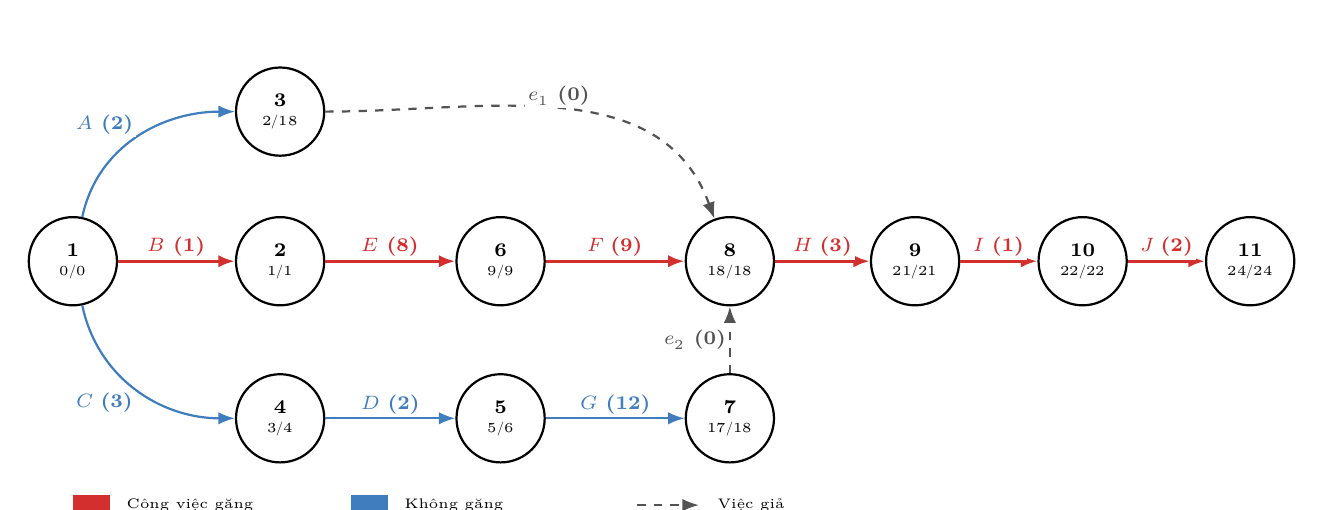
\begin{tikzpicture}[x=1.12cm,y=0.95cm]
  \node[event] (p1)  at (0.00,1.55) {1\\[-1pt]{\tiny\normalfont $0/0$}};
  \node[event] (p3)  at (2.35,3.55) {3\\[-1pt]{\tiny\normalfont $2/18$}};
  \node[event] (p2)  at (2.35,1.55) {2\\[-1pt]{\tiny\normalfont $1/1$}};
  \node[event] (p4)  at (2.35,-0.55) {4\\[-1pt]{\tiny\normalfont $3/4$}};
  \node[event] (p6)  at (4.85,1.55) {6\\[-1pt]{\tiny\normalfont $9/9$}};
  \node[event] (p5)  at (4.85,-0.55) {5\\[-1pt]{\tiny\normalfont $5/6$}};
  \node[event] (p8)  at (7.45,1.55) {8\\[-1pt]{\tiny\normalfont $18/18$}};
  \node[event] (p7)  at (7.45,-0.55) {7\\[-1pt]{\tiny\normalfont $17/18$}};
  \node[event] (p9)  at (9.55,1.55) {9\\[-1pt]{\tiny\normalfont $21/21$}};
  \node[event] (p10) at (11.45,1.55) {10\\[-1pt]{\tiny\normalfont $22/22$}};
  \node[event] (p11) at (13.35,1.55) {11\\[-1pt]{\tiny\normalfont $24/24$}};

  \draw[arc] (p1) to[out=78,in=180] node[arclabel,above left] {$A$ (2)} (p3);
  \draw[criticalarc] (p1) -- node[arclabel,above] {$B$ (1)} (p2);
  \draw[arc] (p1) to[out=-78,in=180] node[arclabel,below left] {$C$ (3)} (p4);
  \draw[criticalarc] (p2) -- node[arclabel,above] {$E$ (8)} (p6);
  \draw[arc] (p4) -- node[arclabel,above] {$D$ (2)} (p5);
  \draw[arc] (p5) -- node[arclabel,above] {$G$ (12)} (p7);
  \draw[criticalarc] (p6) -- node[arclabel,above] {$F$ (9)} (p8);
  \draw[dummyarc] (p3) to[out=0,in=110] node[arclabel,above] {$e_1$ (0)} (p8);
  \draw[dummyarc] (p7) -- node[arclabel,left] {$e_2$ (0)} (p8);
  \draw[criticalarc] (p8) -- node[arclabel,above] {$H$ (3)} (p9);
  \draw[criticalarc] (p9) -- node[arclabel,above] {$I$ (1)} (p10);
  \draw[criticalarc] (p10) -- node[arclabel,above] {$J$ (2)} (p11);

  \fill[criticalbar] (0.00,-1.85) rectangle +(0.42,0.28);
  \node[anchor=west,font=\tiny] at (0.50,-1.71) {Công việc găng};
  \fill[normalbar] (3.15,-1.85) rectangle +(0.42,0.28);
  \node[anchor=west,font=\tiny] at (3.65,-1.71) {Không găng};
  \draw[dummyarc] (6.40,-1.71) -- +(0.70,0);
  \node[anchor=west,font=\tiny] at (7.20,-1.71) {Việc giả};
\end{tikzpicture}}
\caption{Mạng PERT. Đường găng $B$--$E$--$F$--$H$--$I$--$J$.}
\end{figure}

\paragraph{b. Chỉ tiêu các sự kiện.}
Tính tiến: $t_s(j)=\max_{i\rightarrow j}\{t_s(i)+d_{ij}\}$, $t_s(1)=0$.
Tính lùi: $t_m(i)=\min_{i\rightarrow j}\{t_m(j)-d_{ij}\}$, $t_m(11)=t_s(11)$.
Dự trữ đỉnh $R(i)=t_m(i)-t_s(i)$; đỉnh găng khi $R=0$.

{\small
\begin{minipage}[t]{0.49\textwidth}
\textbf{Tiến}\\[1pt]
$t_s(1)=0$\\
$t_s(2)=0+1=1$\\
$t_s(3)=0+2=2$\\
$t_s(4)=0+3=3$\\
$t_s(5)=3+2=5$\\
$t_s(6)=1+8=9$\\
$t_s(7)=5+12=17$\\
$t_s(8)=\max\{2+0,\ 9+9,\ 17+0\}=18$\\
$t_s(9)=18+3=21$\\
$t_s(10)=21+1=22$\\
$t_s(11)=22+2=24$
\end{minipage}
\hfill
\begin{minipage}[t]{0.49\textwidth}
\textbf{Lùi}\\[1pt]
$t_m(11)=24$\\
$t_m(10)=24-2=22$\\
$t_m(9)=22-1=21$\\
$t_m(8)=21-3=18$\\
$t_m(7)=18-0=18$\\
$t_m(6)=18-9=9$\\
$t_m(5)=18-12=6$\\
$t_m(4)=6-2=4$\\
$t_m(3)=18-0=18$\\
$t_m(2)=9-8=1$\\
$t_m(1)=\min\{18-2,\ 1-1,\ 4-3\}=0$
\end{minipage}
}

\begin{table}[H]\centering
\caption{Thời điểm sớm, muộn và dự trữ các sự kiện}
\small
\begin{tabular}{c|rrrrrrrrrrr}
\toprule
Sự kiện $i$ & 1 & 2 & 3 & 4 & 5 & 6 & 7 & 8 & 9 & 10 & 11\\
\midrule
$t_s(i)$ & 0 & 1 & 2 & 3 & 5 & 9 & 17 & 18 & 21 & 22 & 24\\
$t_m(i)$ & 0 & 1 & 18 & 4 & 6 & 9 & 18 & 18 & 21 & 22 & 24\\
$R(i)$   & 0 & 0 & 16 & 1 & 1 & 0 & 1 & 0 & 0 & 0 & 0\\
\bottomrule
\end{tabular}
\end{table}

Đỉnh găng: $1,2,6,8,9,10,11$.
Thời gian sớm nhất hoàn thành dự án: $T=t_s(11)=t_m(11)=\mathbf{24}$ ngày.

\paragraph{Các yếu tố thời gian của công việc.}
Với cung $i\rightarrow j$:
$ES=t_s(i)$, $EF=t_s(i)+d$, $LS=t_m(j)-d$, $LF=t_m(j)$,
$TF=t_m(j)-t_s(i)-d$,
$FF=t_s(j)-t_s(i)-d$,
$IF=\max\{0,\ t_s(j)-t_m(i)-d\}$.

\begin{table}[H]\centering
\caption{Chỉ tiêu thời gian các công việc}
\small
\begin{tabular}{c|c|c|rr|rr|rrr}
\toprule
\textbf{CV} & $i\!\rightarrow\!j$ & $d$ & ES & EF & LS & LF & TF & FF & IF\\
\midrule
$A$ & $1\rightarrow 3$ & 2 & 0 & 2 & 16 & 18 & 16 & 0 & 0\\
$B$ & $1\rightarrow 2$ & 1 & 0 & 1 & 0 & 1 & \textbf{0} & 0 & 0\\
$C$ & $1\rightarrow 4$ & 3 & 0 & 3 & 1 & 4 & 1 & 0 & 0\\
$D$ & $4\rightarrow 5$ & 2 & 3 & 5 & 4 & 6 & 1 & 0 & 0\\
$E$ & $2\rightarrow 6$ & 8 & 1 & 9 & 1 & 9 & \textbf{0} & 0 & 0\\
$F$ & $6\rightarrow 8$ & 9 & 9 & 18 & 9 & 18 & \textbf{0} & 0 & 0\\
$G$ & $5\rightarrow 7$ & 12 & 5 & 17 & 6 & 18 & 1 & 0 & 0\\
$H$ & $8\rightarrow 9$ & 3 & 18 & 21 & 18 & 21 & \textbf{0} & 0 & 0\\
$I$ & $9\rightarrow 10$ & 1 & 21 & 22 & 21 & 22 & \textbf{0} & 0 & 0\\
$J$ & $10\rightarrow 11$ & 2 & 22 & 24 & 22 & 24 & \textbf{0} & 0 & 0\\
\bottomrule
\end{tabular}
\end{table}

\paragraph{Đường găng.}
Công việc găng khi $TF=0$: $B,E,F,H,I,J$.
Đối chiếu các đường đi từ 1 đến 11:
\begin{itemize}
  \itemsep=1pt
  \item $A$--$e_1$--$H$--$I$--$J$: $2+0+3+1+2=8$
  \item $B$--$E$--$F$--$H$--$I$--$J$: $1+8+9+3+1+2=\mathbf{24}$
  \item $C$--$D$--$G$--$e_2$--$H$--$I$--$J$: $3+2+12+0+3+1+2=23$
\end{itemize}
\[
  \boxed{B\text{--}E\text{--}F\text{--}H\text{--}I\text{--}J\qquad (1+8+9+3+1+2=24\ \text{ngày})}
\]

Công việc không găng: $A$ ($TF=16$), $C,D,G$ ($TF=1$).
Dự trữ độc lập $IF=0$ với mọi công việc, nên không thể đồng thời kéo dài tất cả công việc không găng thêm ngày nào mà không đụng tiến độ: chuỗi $C$--$D$--$G$ chỉ còn 1 ngày dự trữ chung.

\end{document}
